\section{Multirate Systems}\label{sec:p3}

\begin{enumerate}[(a)]
\item Let $u[n]$ be the output after downsampling and $v[n]$ be the output after convolving with $g$.
\begin{align*}
	U(z) &= \frac{1}{2} \sum_{k=0}^{1}X\left(e^{-j\frac{2\pi k}{2}} z^{1/2}\right)\\
	&= \frac{1}{2} \left(X(z^{1/2} + X(e^{-j\pi}z^{1/2}))\right) \\
	V(z) &= G(z)U(z) \\
	Y(z) &= V(z^3) \\
	&= G(z^3)U(z^3) \\
	&= \frac{1}{2} \left(X(z^{3/2} + X(e^{-j\pi}z^{3/2}))\right)
\end{align*}

\item $x[n] = q(nT)$ is the same as downsampling by $T$, so $u[z]$ is obtained by downsampling $q(t)$ by $2T$. Therefore
\begin{align*}
	U(\omega) &= \frac{1}{2T} \sum_{k=0}^{2T-1} Q\left(\frac{\omega-2\pi k}{2T}\right) \\
	V(\omega) &= G(\omega)U(\omega) \\
	Y(\omega) &= V(3\omega) \\
	&= G(3\omega)U(3\omega) \\
	&= \frac{G(3\omega)}{2T} \sum_{k=0}^{2T-1} Q\left(\frac{3\omega-2\pi k}{2T}\right)
\end{align*}

Since $q \in BL[-\frac{\pi}{T}, \frac{\pi}{T}]$ and the sampling rate $\frac{1}{T}$, we have the setting in Figure \ref{fig:p3}
\begin{figure}[htbp]
	\centering
	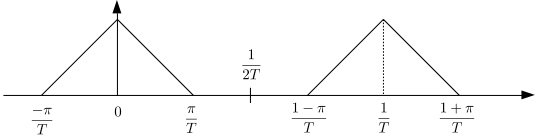
\includegraphics[width=\textwidth]{images/p3}
	\caption{Sampling $q \in BL[-\frac{\pi}{T}, \frac{\pi}{T}]$ with sampling rate of $\frac{1}{T}$}
	\label{fig:p3}
\end{figure}
To avoiud aliasing, we need $\frac{\pi}{T} < \frac{1}{2T} \Leftrightarrow \frac{2\pi-1}{T} < 0$, which cannot satisfy. Therefore, $q$ cannot avoid aliasing after sampling.
\end{enumerate}